\documentclass{elsarticle}

%=============== Packages ===================%
\usepackage{amsmath}
\usepackage{amssymb}
\usepackage{amsfonts}
\usepackage{graphicx}
\usepackage{colortbl}
\usepackage{url}
\usepackage{tikz}
\usepackage[ruled]{algorithm2e}
\usepackage{flushend}
\usepackage{footnote}
\usepackage{threeparttable}
\usepackage[justification=centering]{caption}
\usepackage{subcaption}
\usepackage[caption=false,font=footnotesize]{subfig}
\usepackage{amsthm}
\usepackage{floatrow}

\newtheorem{mydef}{Definition}
\theoremstyle{definition}

%=============== Preamble ===================%
\journal{Book on Plan, Activity, and Intent Recognition}

\begin{document}
\begin{frontmatter}

\title{Stream Sequence Mining for Human Activity Discovery}

\author{Parisa Rashidi}
\ead{parisa.rashidi@northwestern.edu}
\address{Biomedical Informatics Division, \\ Health and Engineering Center, \\ Northwestern University, \\ Chicago, IL, US}

%=============== Abstract ==================%

\begin{keyword}
Activity Discovery \sep Activity Recognition \sep Unsupervised Learning \sep Sequence Mining \sep Stream Mining
\end{keyword}

\end{frontmatter}
%=============== Content ===================%

\textbf{todo: re-save figures in pdf format}
\section{Methods}
\subsection{Standardizing start times}
Most pain scores in the data file begin shortly after surgery, with about 80\% starting within two hours post-operation. However, there is a non-trivial subset of patients whose pain score recordings started up to several days after their surgeries, as shown in Figure \ref{fig:start_times}.

\begin{figure}[h]
        \begin{subfigure}{0.5\textwidth}
                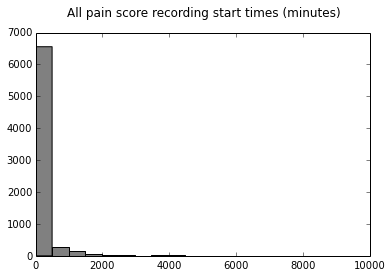
\includegraphics[width=\textwidth]{Figures/pain_score_start_times.png}
                \caption{Normal scale}
                \label{fig:start_times_normal}
        \end{subfigure}\begin{subfigure}{0.5\textwidth}
                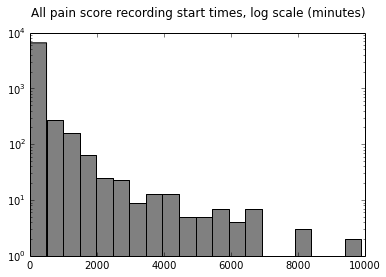
\includegraphics[width=\textwidth]{Figures/pain_score_start_times_log.png}
                \caption{Log scale}
                \label{fig:start_times_log}
        \end{subfigure}
        \caption{Histograms of all pain score start times in minutes, both normal and logarithmic scales}\label{fig:start_times}
\end{figure}

In the interest of analyzing pain profiles along a standard post-operation time interval, data was disregarded for those patients whose pain scores were recorded starting more than two hours after their procedure. This operation retained 80\% of the original data set. Figure \ref{fig:start_times_pruned} shows the set of start times less than two hours post-operation.

\begin{figure}[h]
        \begin{subfigure}{0.5\textwidth}
                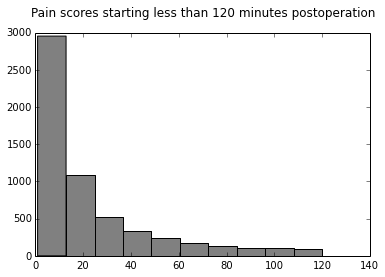
\includegraphics[width=\textwidth]{Figures/pain_score_start_times_lte2hours.png}
                \caption{Normal scale}
                \label{fig:start_times_pruned_normal}
        \end{subfigure}\begin{subfigure}{0.5\textwidth}
                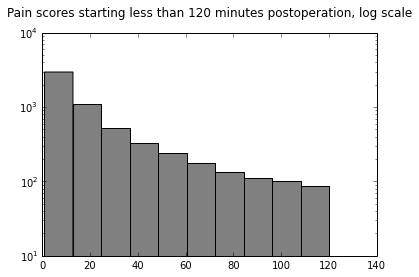
\includegraphics[width=\textwidth]{Figures/pain_score_start_times_lte2hours_log.png}
                \caption{Log scale}
                \label{fig:start_times_pruned_log}
        \end{subfigure}
        \caption{Histograms of all pain score start times less than 120 minutes, both normal and logarithmic scales}\label{fig:start_times_pruned}
\end{figure} 
\subsection{Interpolation}
Let $p$ refer to an arbitrary patient whose pain score records started less than two hours post-operation. Since pain scores were recorded at inconsistent intervals, it is necessary to standardize them to consistent intervals. Ten minutes was chosen as the standard interval between scores, and recorded scores were linearly interpolated  and estimated for these periods. Figure \ref{fig:interpolation} illustrates the transformation from sample recorded scores, \eqref{eqn:recorded_scores}, to interpolated scores, \eqref{eqn:interpolated_scores} (rounded to the hundredths place for display purposes).

\begin{equation}\label{eqn:recorded_scores}
    recorded=(3\ minutes: 4, 24\ minutes: 8, 45\ minutes: 4, 100\ minutes: 2)
\end{equation}

\begin{equation}\label{eqn:interpolated_scores}
\begin{split}
    interpolated=(&3\ minutes:4.0, 13\ minutes:5.9, 23\ minutes:7.8,\\
                  &33\ minutes:6.3, 43\ minutes:4.4, 53\ minutes:3.7,\\
                  &63\ minutes:3.3, 73\ minutes:3.0, 83\ minutes:2.6,\\
                  &93\ minutes:2.0)
\end{split}
\end{equation}

\begin{figure}[h]
  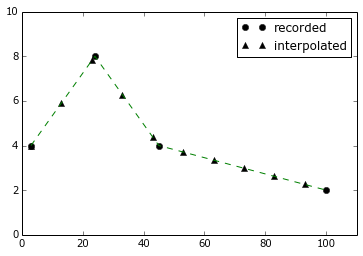
\includegraphics[scale=0.4]{./Figures/interpolation.png}\\
  \caption{Illustration of interpolation procedure. Recorded pain scores are connected via a linear function of time from which interpolated scores are predicted at consistent, ten-minute intervals.}\label{fig:interpolation}
\end{figure}

Denote patient $p$'s time series of 10-minute interpolated pain scores as $\tilde{S}=(s_1,...,s_d)$, where the $t$'th item is the estimated pain score $10(t-1)$ minutes past the first recorded score, and $d=floor\left(\frac{max(recording time)}{10}\right)$. So $s_1$ is the first pain score recorded for that patient with subsequent elements estimated from linear interpolation, and $d$ is the index of the last available data point estimated from interpolation without forecasting past the last recorded pain score. For the example interpolated values in \eqref{eqn:interpolated_scores}, $\tilde{S}=(4.0, 5.9, 7.8, 6.3, 4.4, 3.7, 3.3, 3.0, 2.6, 2.3)$. 
\subsection{Calculating  motif occurrences}
Each motif of length $l$ is represented by a vector of alphabet letter indices $\left(k_1,k_2,...,k_l\right)$, 1-based such that motif \emph{adb} would be $\left(1,4,2\right)$. Define a matrix of motif occurences $M$ from a collection of motifs such that $M_{p,m}$ refers to the occurrence count of motif $m$ within a given SAX sequence representing the post-operative pain scores for patient $p$ (pain scores are linearly interpolated to ten minute increments). For any given motif of length $l$ represented by up to $\beta$ letters of the alphabet, its position in the matrix is defined by Equation \eqref{eqn:motif_position}.

\begin{equation}\label{eqn:motif_position}
    m = 1+\sum\limits_{j=1}^l \left(k_j-1\right)\times\beta^{l-j}
\end{equation}

For example, given a motif such as \emph{adb}, with $\beta=4$ (that is, an alphabet letter selection of $\left\{a,b,c,d\right\}$), then $m=14$. This has the effect of placing the motifs in alphabetical order within the vector $M_{p,.}$. Note that the total number of possible motifs of length $l$ with $\beta$ alphabet letters is $\beta^l$. In our analysis, $l$ was restricted to a value of $2$, and values of $\beta$ were examined along the set $\left\{2,5,10\right\}$.

\subsection{Clustering}
Define multiple clusters of patients $\left(C_{\kappa_1},...,C_{\kappa_n}\right)$ such that $p \in C_{\kappa_i}$, $iif$ criterion $\kappa_i$ describes patient $p$. A given criterion $\kappa$ may specify the patient's gender, age group, surgery type, etc. or include a set of multiple criteria. The relative importance $x_{C_{\kappa},m}$ of motif $m$ to a given cluster $C_{\kappa}$ can therefore be calculated as follows:
\begin{equation}\label{eqn:motif_importance}
    x_{C_\kappa,m} = \frac{\sum\limits_{p \in C_\kappa} M_{p,m}}{\sum\limits_{p \in C_\kappa} \sum\limits_{m} M_{p,m}}
\end{equation}
In other words, the relative importance is equal to the occurence count for motif $m$ within the recoveries of all patients in the cluster divided by the total occurence count for all motifs within those recoveries.

Note that a patient could hypothetically be assigned to multiple clusters if, for example, the analysis looked at a feature whose value changed during the course of data collection (such as the patient started on a new medication during the course of his/her recovery). While this is potentially an area where the procedure could be improved, the data file does not appear to exhibit this behavior. Feature values were static for any given patient, and thus there would be no duplication between clusters.
\subsection{Normalizing}
In addition to comparing all motif importance values within the same cluster, the goal is also to compare individual motifs importance values across clusters. As such it is necessary to normalize $x_{C_\kappa,m}$ in order to elucidate subtle differences across all relevant cluster criteria. One simple and effective option is to use the standard score $z_{C_\kappa,m}$.

In a realistic analysis, the number of clusters is generally very small. For example, if $\kappa \in \left\{patient\ is\ taking\ an\ SSRI,patient\ is\ not\ taking\ an\ SSRI\right\}$, then the mean $\mu_{.,m}$ and standard deviation $\sigma_{.,m}$ of importance values for motif $m$ across all clusters in the analysis only take into account two values for $x_{C_\kappa,m}$, hardly enough to calculate a useful standard score. Therefore, instead of normalizing values of $x_{.,m}$ directly against each other, values of $x_{C_\kappa,m}$ were normalized against the random distribution $x_{C_\kappa,m}^*$, bootstrapped by taking a sufficiently large number of random samples of relative importance values. For any given cluster $C_\kappa$ and motif $m$,

\begin{enumerate}
  \item Let $|C_\kappa|$ be the number of patients in $C_\kappa$.
  \item Take some arbitrarily large number $n$ (say, 1000) of random samples $\left(C_{r_1},...,C_{r_n}\right)$ so that each sample represents a cluster of $|C_\kappa|$ patients independently chosen from $\left\{all\ patients\right\}$ with replacement and uniform probability of being chosen.
  \item For each sample $C_r$, calculate the relative motif importance $x_{C_r,m}$. Refer to this new set, $\left\{x_{C_{r_1},m}, x_{C_{r_2},m}, ..., x_{C_{r_n},m}\right\}$, as $x_{C_\kappa,m}^*$. Ideally $x_{C_\kappa,m}^*$ will resemble a normal distribution. As figure \ref{fig:5x5_hist} shows, this appears to be the case from the data set for example values of $n_r=1000$, $|C_\kappa|=100$, and $\beta=5$. Although, this is not necessarily the case for every $x_{C_\kappa,m}^*$ when $\beta$ is sufficiently large or $|C_\kappa|$ is sufficiently small. Figure \ref{fig:10x10_hist_ck100} shows $x_{C_\kappa,m}^*$ histograms when $n_r=1000$, $|C_\kappa|=100$, and $\beta=10$. Near two of the corners $x_{C_\kappa,m}^*$ values hover around 0. The reason is that instances of such drastic jumps in pain scores (\emph{j} to \emph{a} or \emph{a} to \emph{j}) are relatively rare. For practical purposes, the visual effect on the final icons as well as the effect on sorting the icons is negligible, so this small source of normalization error is acceptable. However, figure \ref{fig:10x10_hist_ck2} shows $x_{C_\kappa,m}^*$ histograms when $n_r=1000$, $|C_\kappa|=2$, and $\beta=10$. Data calculated for these parameters are clearly not normal, which is unsurprising given that the numerator in $x_{C_\kappa,m}$ expresses additive behavior over potentially rare events; that is, the sum of the number of times patients in a given cluster went from one normalized pain level to another. Therefore, in this analysis, which limited $\beta$ to a maximum value of 10, only clusters which contained at least 100 patients ($|C_\kappa|\geq100$) were considered. As it turns out, most interesting clusters have several hundred patients, so this limit is rarely an issue. In the future, however, other probability distributions may prove useful in analyzing these smaller clusters.
\begin{figure}
  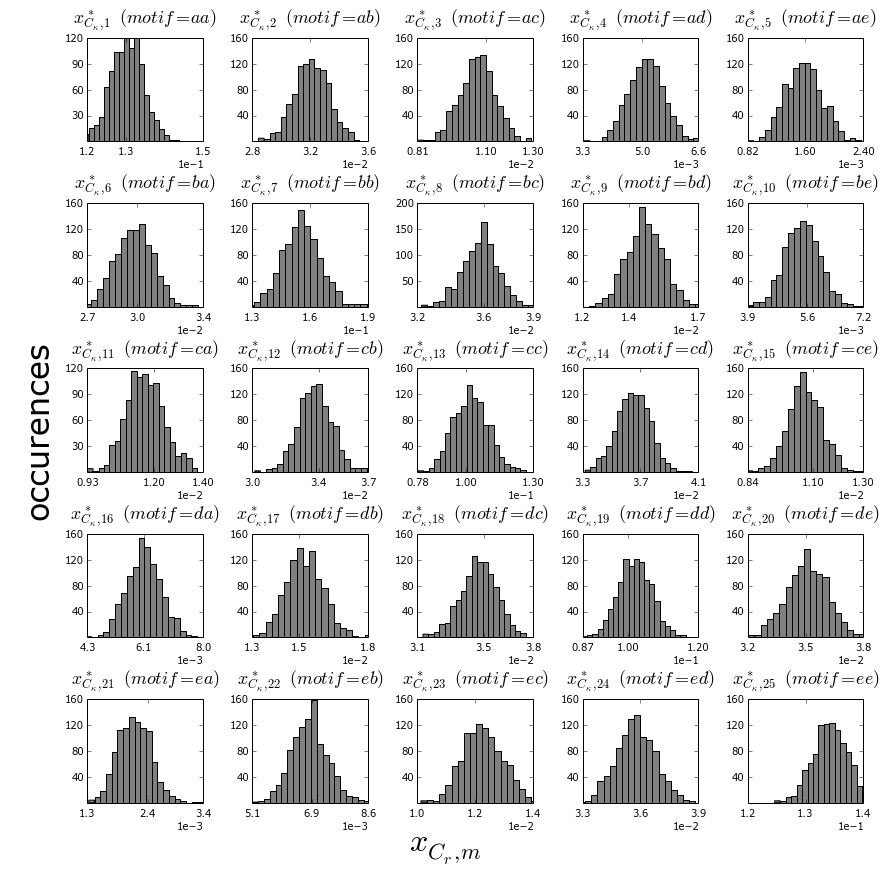
\includegraphics[scale=0.35]{./Figures/5x5hist.png}\\
  \caption{Histograms of resampled importance values for each motif, with parameters $n_r=1000$, $|C_\kappa|=100$, and $\beta=5$. Demonstrates ideal normal behavior of the simulated importance value distributions.}\label{fig:5x5_hist}
\end{figure}
\begin{figure}
  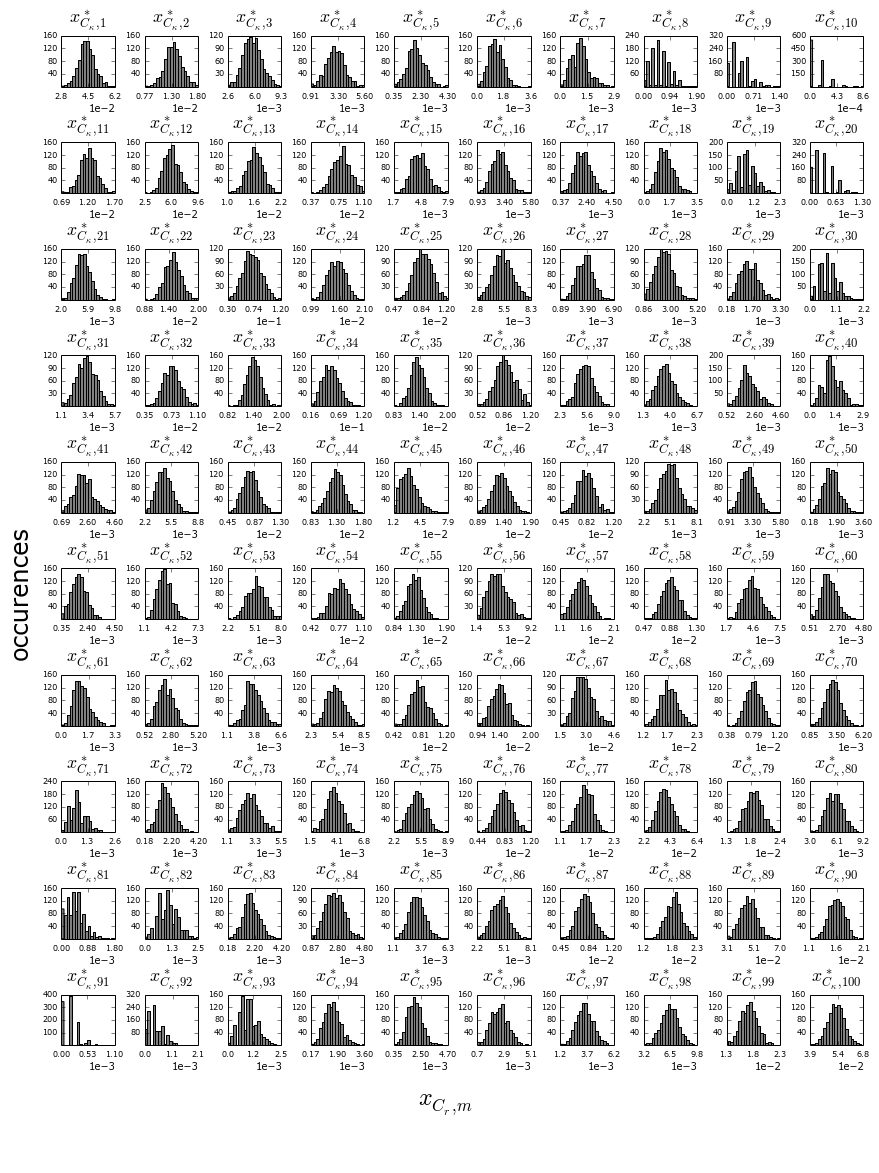
\includegraphics[scale=0.35]{./Figures/10x10hist_ck100.png}\\
  \caption{Histograms of resampled importance values for each motif, with parameters $n_r=1000$, $|C_\kappa|=100$, and $\beta=10$. Demonstrates slight deviation from normal behavior around the upper-right and lower-left corners.}\label{fig:10x10_hist_ck100}
\end{figure}
\begin{figure}
  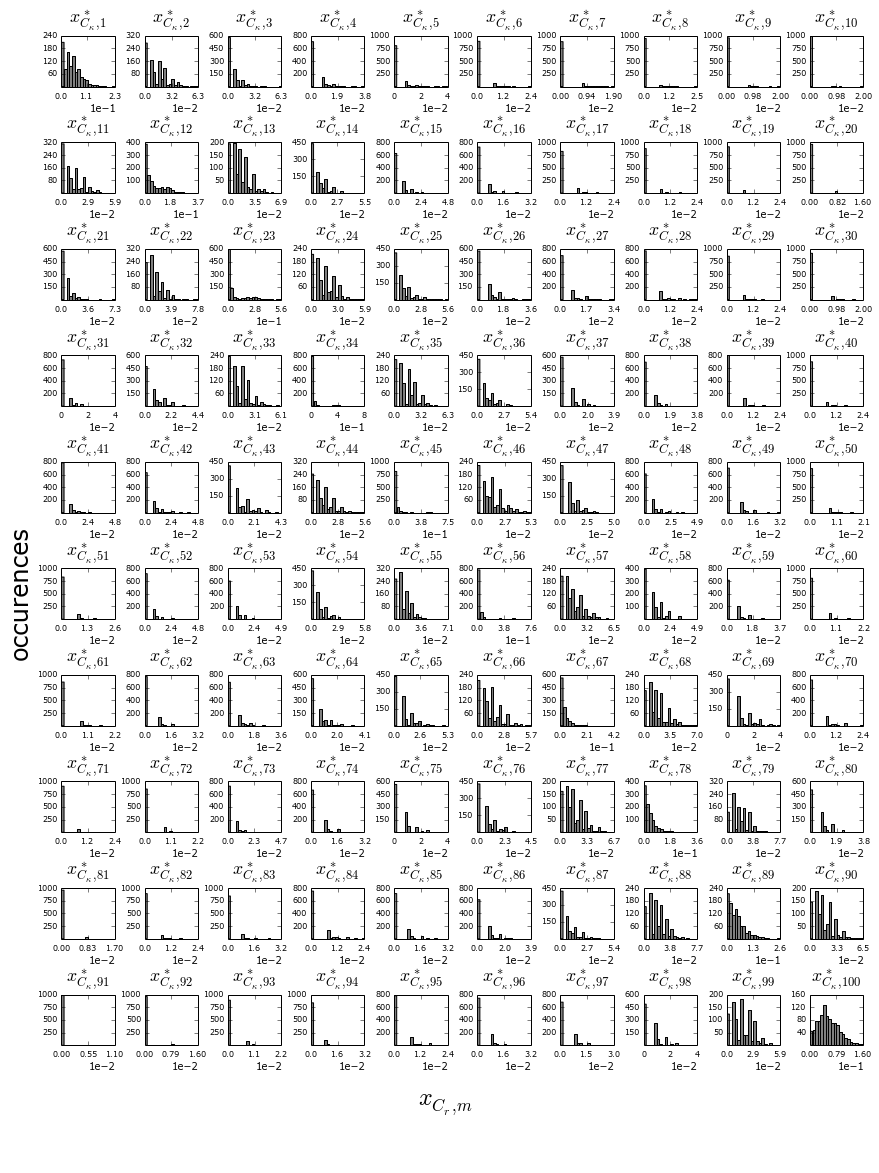
\includegraphics[scale=0.35]{./Figures/10x10hist_ck2.png}\\
  \caption{Histograms of resampled importance values for each motif, with parameters $n_r=1000$, $|C_\kappa|=2$, and $\beta=10$. Demonstrates collapse of normality expectation and necessitates the restriction on cluster sizes of less than 100 patients.}\label{fig:10x10_hist_ck2}
\end{figure}
  \item From $x_{C_\kappa,m}^*$, calculate the mean $\mu_{C_\kappa,m}$ and standard deviation $\sigma_{C_\kappa,m}$. The normalized value of $x_{C_\kappa,m}$ is therefore the standard score

\begin{equation}\label{eqn:normalize_motif_importance}
    z_{C_\kappa,m}=\frac{x_{C_\kappa,m}-\mu_{C_\kappa,m}}{\sigma_{C_\kappa,m}}
\end{equation}

      The vertical lines in figure \ref{fig:5x5hist_standardscore} represent values for $z_{C_\kappa,m}$ plotted against histograms for standard scores of all values in $x_{C_\kappa,m}^*$; that is, equation \eqref{eqn:normalize_motif_importance} applied to all sampled points in $x_{C_\kappa,m}^*$ (creating a derived distribution, $z_{C_\kappa,m}^*$). Specifically, these data represent parameter values $\beta=5$, $n_r=1000$, and $\kappa=$``\emph{patient underwent cardiovascular surgery}'' (PrimaryCPTCodeCategory2 = \emph{Cardiovascular}), a cluster which contains 582 patients ($|C_\kappa|=582$).

\begin{figure}
  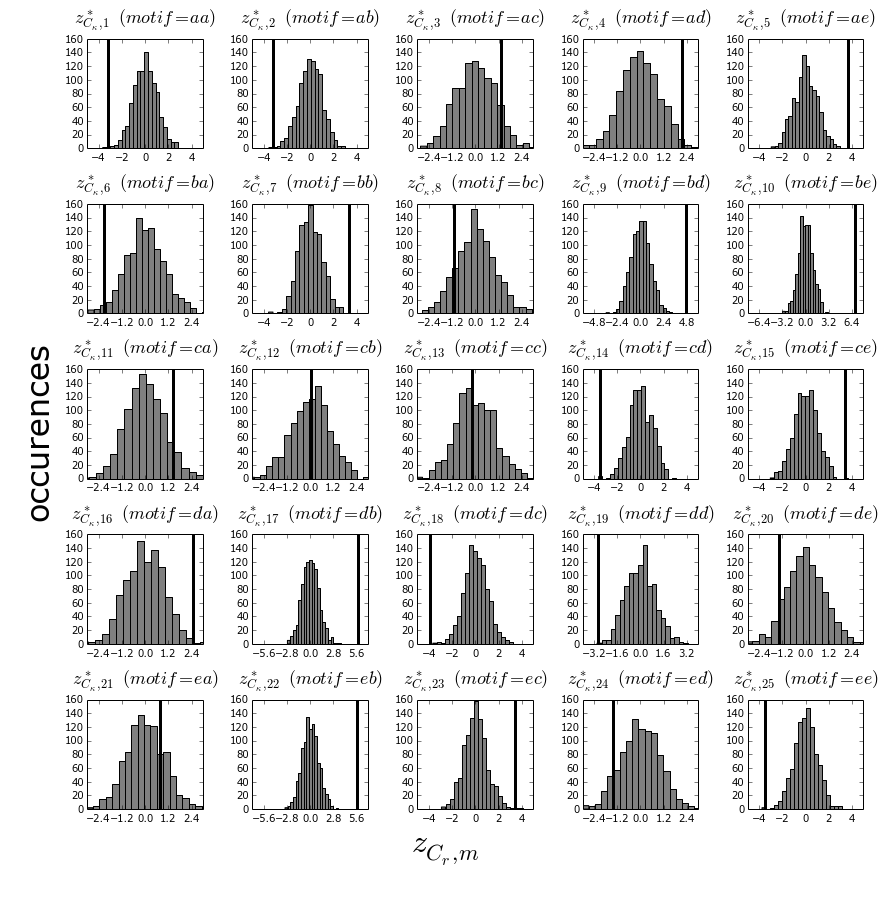
\includegraphics[scale=0.35]{./Figures/5x5hist_standardscore.png}\\
  \caption{Histograms of resampled importance values for each motif, converted to their standard score, with parameters $n_r=1000$, $|C_\kappa|=100$, and $\beta=5$. Vertical lines correspond to normalized importance values for the cluster of patients that underwent cardiovascular surgery.}\label{fig:5x5hist_standardscore}
\end{figure}

\end{enumerate} 
\subsection{Generating intelligent icons}
Let $z_{C_{\kappa},.}$ be the vector of normalized importance values within cluster $C_\kappa$ for all motifs. As noted earlier, because our analysis was limited to length two motifs, the total number of motifs is $\beta^2$. Therefore $z_{C_{\kappa},.}$ can be reshaped to a square icon with side lengths $\beta$. The function named reshape() - implemented in either Matlab or Numpy - was used with $z_{C_{\kappa},.}$ and the number of columns and rows as parameters to generate icon matrices. Reshape() in Matlab orders differently than in Numpy, but specifying to use Fortran order in Numpy recreates Matlab behavior. However, since our analysis was done in Numpy, for the sake of convenience Numpy's default behavior was used, which lays motifs out along the icon as shown in figure \ref{fig:example_icon}. Pixel colors correspond to $z_{C_{\kappa},m}$ values and are capped at $[-3,3]$, corresponding to $-3$ and $+3$ standard deviations from the mean.

\begin{figure}[h]
  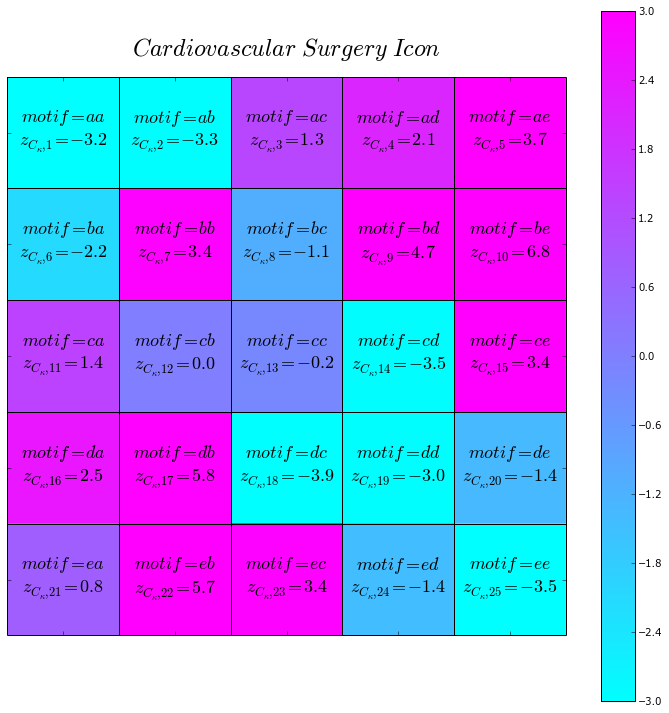
\includegraphics[scale=0.35]{./Figures/example_icon.png}\\
  \caption{Sample icon for the cluster of patients that underwent cardiovascular surgery, with text overlaying each pixel describing how the color was calculated. \textbf{Needed: redo this once decision is made on normalized/unnormalized SAX}}\label{fig:example_icon}
\end{figure} 
\subsection{Sorting icons by similarity}
For larger numbers of clusters, it is often useful to determine which clusters are most similar to each other. One option of doing so is to use cosine similarity. For any two clusters $C_{\kappa_1}$ and $C_{\kappa_2}$,

\begin{equation}\label{eqn:cosine_similarity}
    \begin{split}
    similarity(C_{\kappa_1}, C_{\kappa_2}) &= cos\left(\theta_{C_{\kappa_1}, C_{\kappa_2}}\right) \\
                                           &= \frac{z_{C_1,.} \cdot z_{C_2,.}}{|\!|z_{C_1,.}|\!||\!|z_{C_2,.}|\!|} \\
                                           &= \frac{\sum\nolimits_{m} z_{C_1,m} \times z_{C_2,m} }{ \sum\nolimits_{m} \left(z_{C_1,m}\right)^2 \times \left(z_{C_2,m}\right)^2 }
    \end{split}
\end{equation}

Similarity is thus measured along the interval $[1,-1]$, with $1$ being an exact match and $-1$ being exactly opposite. When plotting icons, a cluster is first chosen and the associated icon plotted. Icons for every other cluster are then plotted in descending similarity from left to right, flowing over to subsequent rows.
 
\section{Examples \textbf{Needed: redo these once decision is made on normalized/unnormalized SAX. Also want more examples}}
\subsection{Surgical procedure}
In this analysis, clusters were defined based on surgical procedure category. Icons are shown in Figure \ref{fig:surgerytype_beta2} corresponding to $\beta=2$, Figure \ref{fig:surgerytype_beta5} to $\beta=5$, and Figure \ref{fig:surgerytype_beta10} to $\beta=10$.

\begin{figure}[h]
  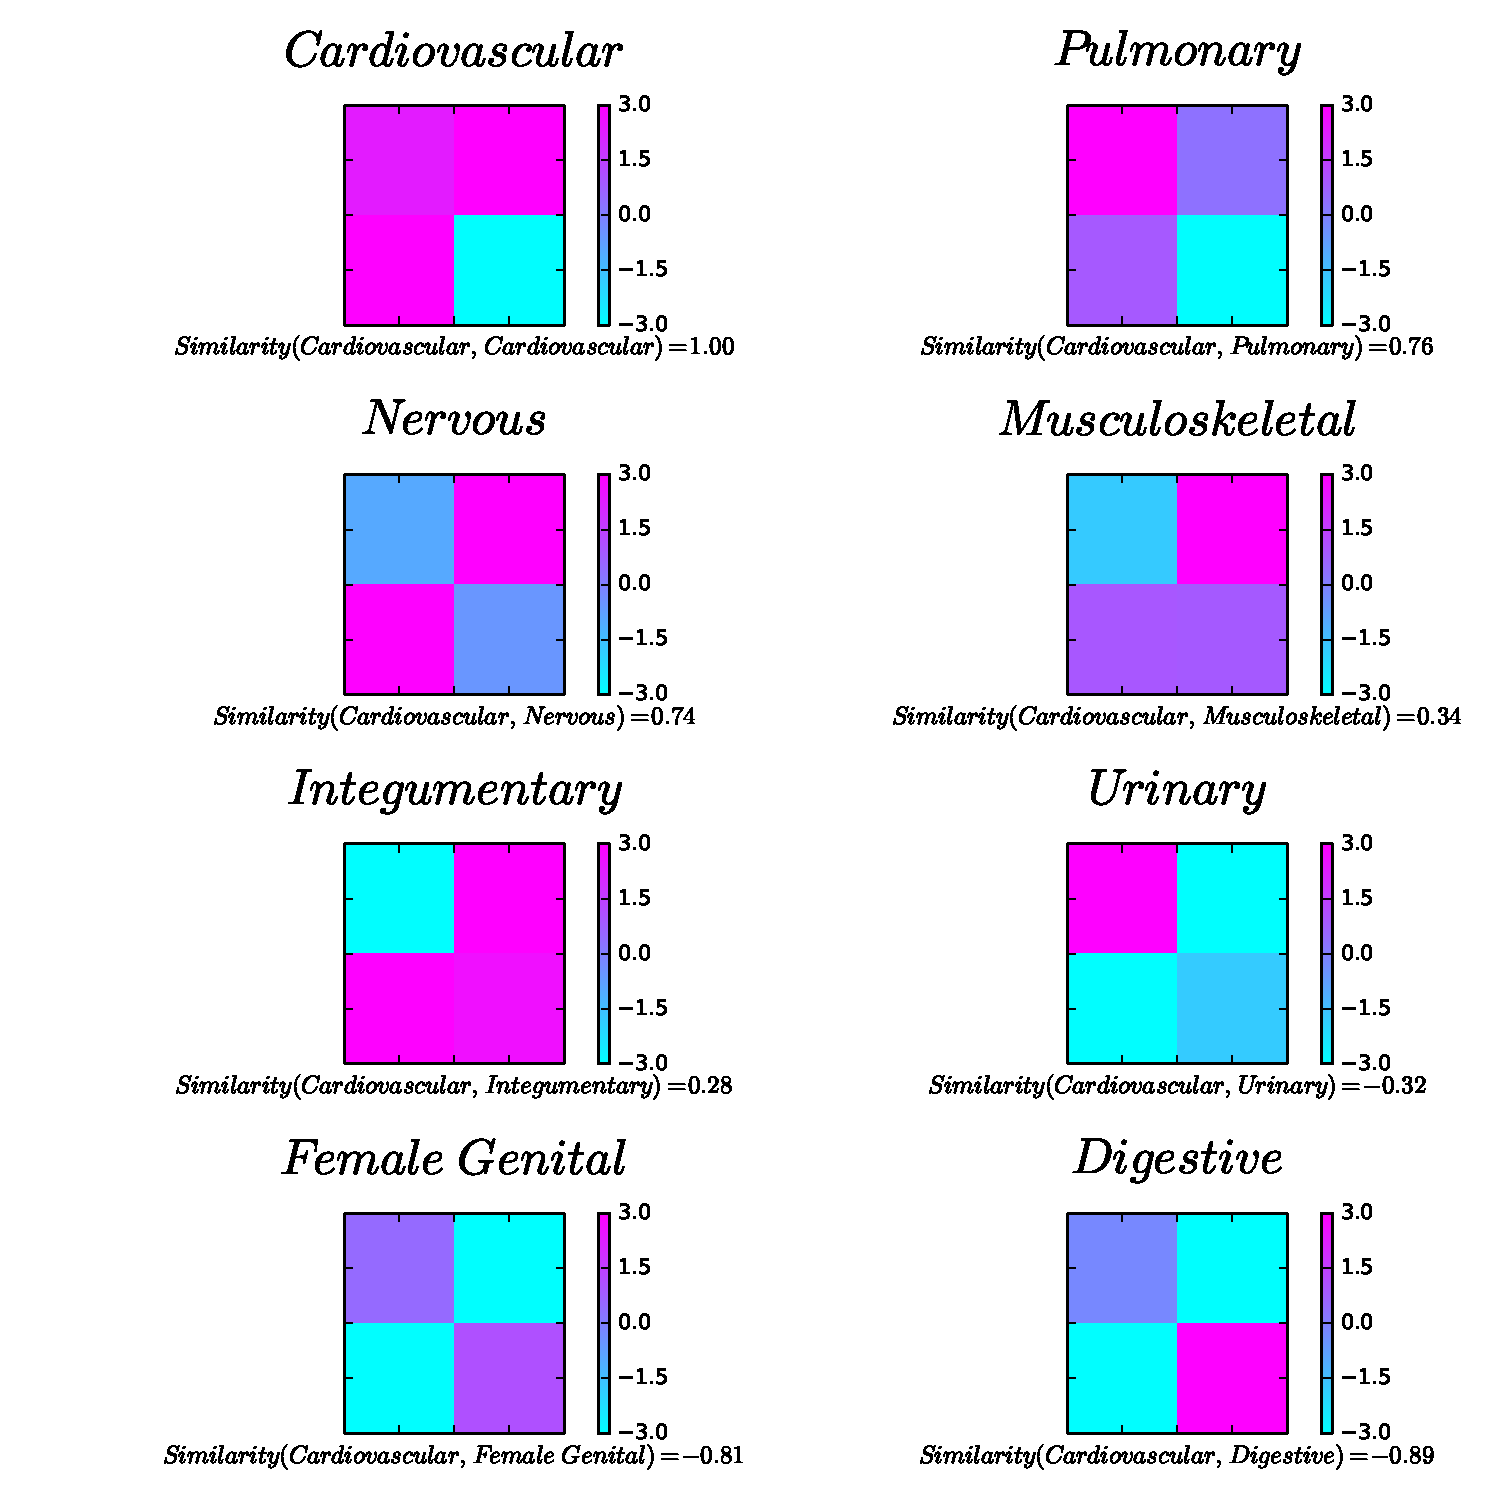
\includegraphics[scale=0.4]{./Figures/surgerytype_beta2.pdf}\\
  \caption{Icons for clusters of patients based on type of surgical procedure, $\beta=2$. Icons are sorted in descending similarity from the cluster of patients who underwent cardiovascular surgery.}\label{fig:surgerytype_beta2}
\end{figure}

\begin{figure}[h]
  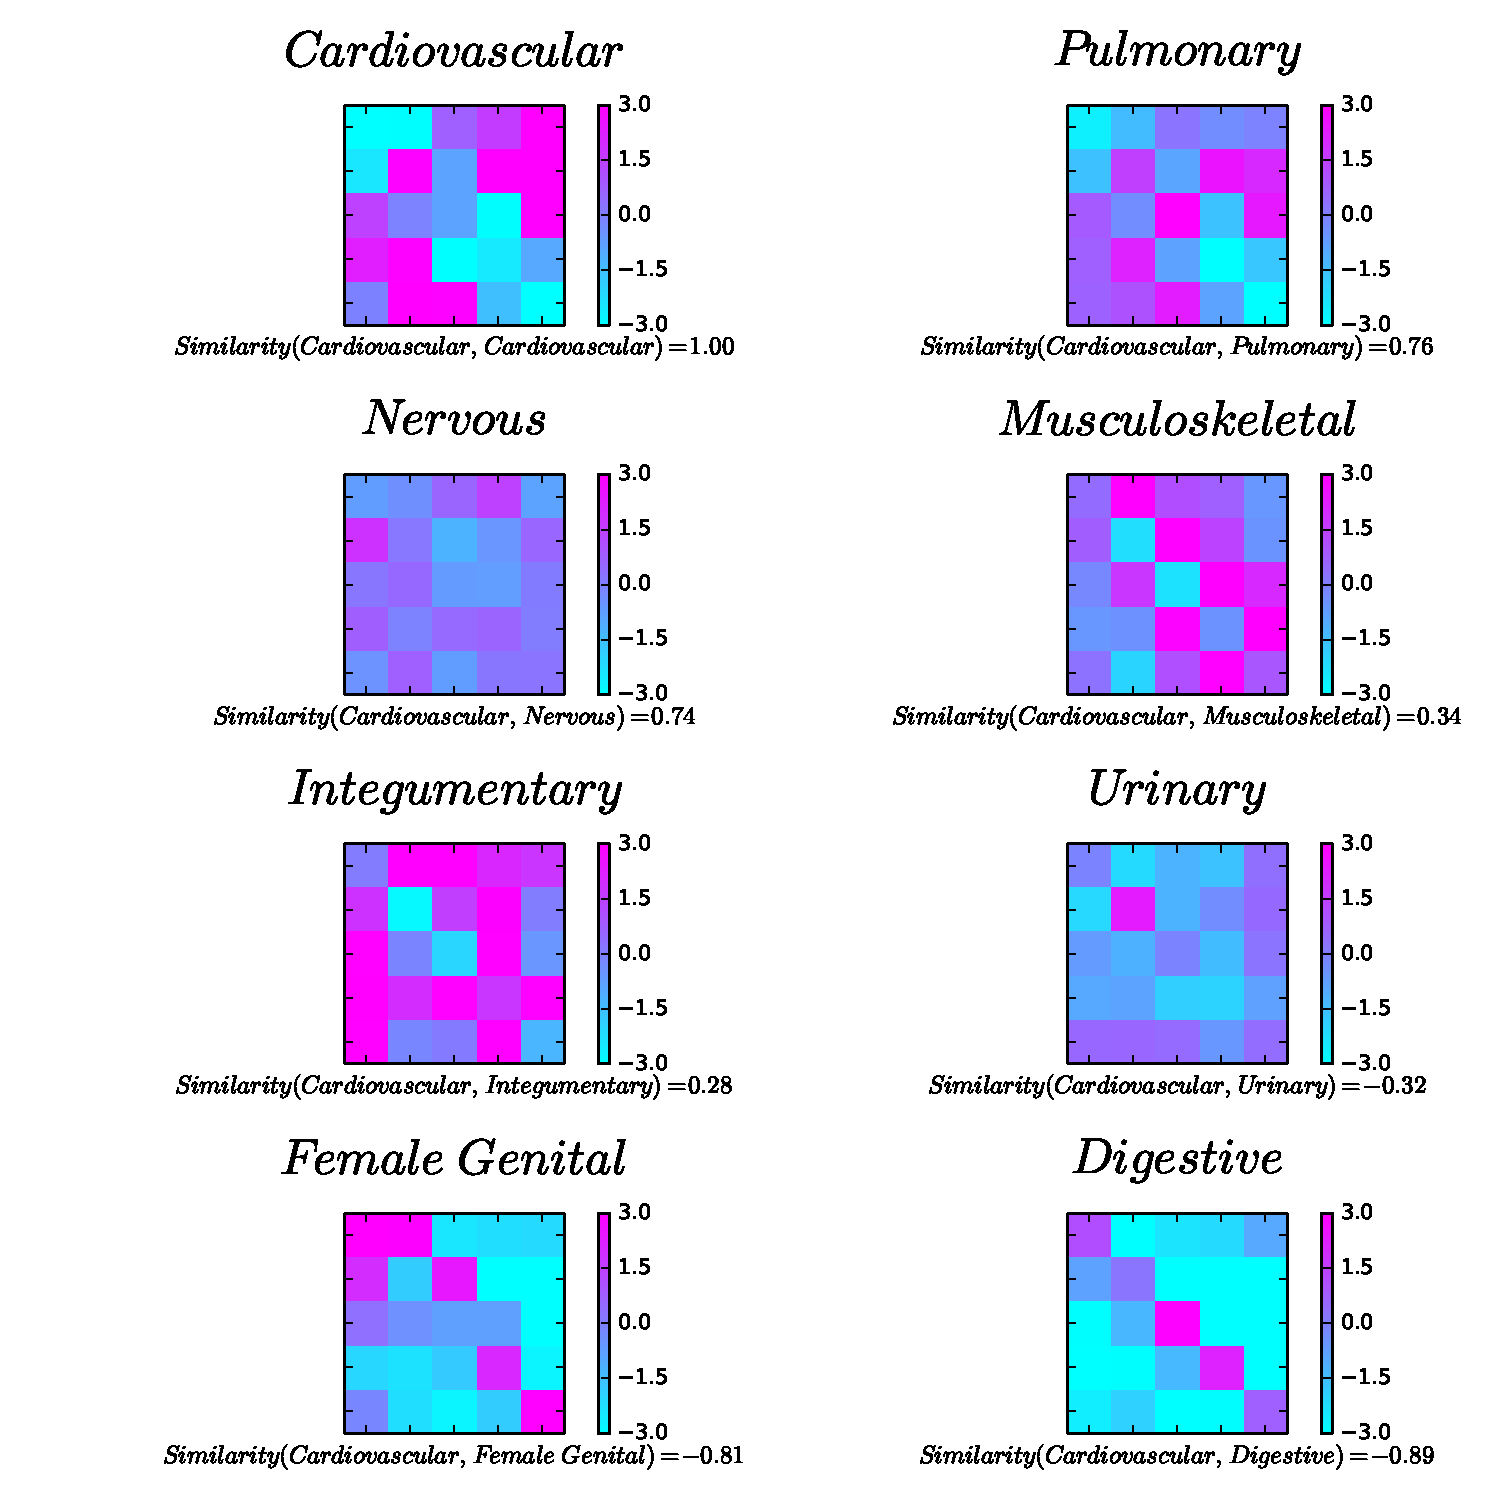
\includegraphics[scale=0.4]{./Figures/surgerytype_beta5.pdf}\\
  \caption{Icons for clusters of patients based on type of surgical procedure, $\beta=5$. Icons are sorted in descending similarity from the cluster of patients who underwent cardiovascular surgery.}\label{fig:surgerytype_beta5}
\end{figure}

\begin{figure}[h]
  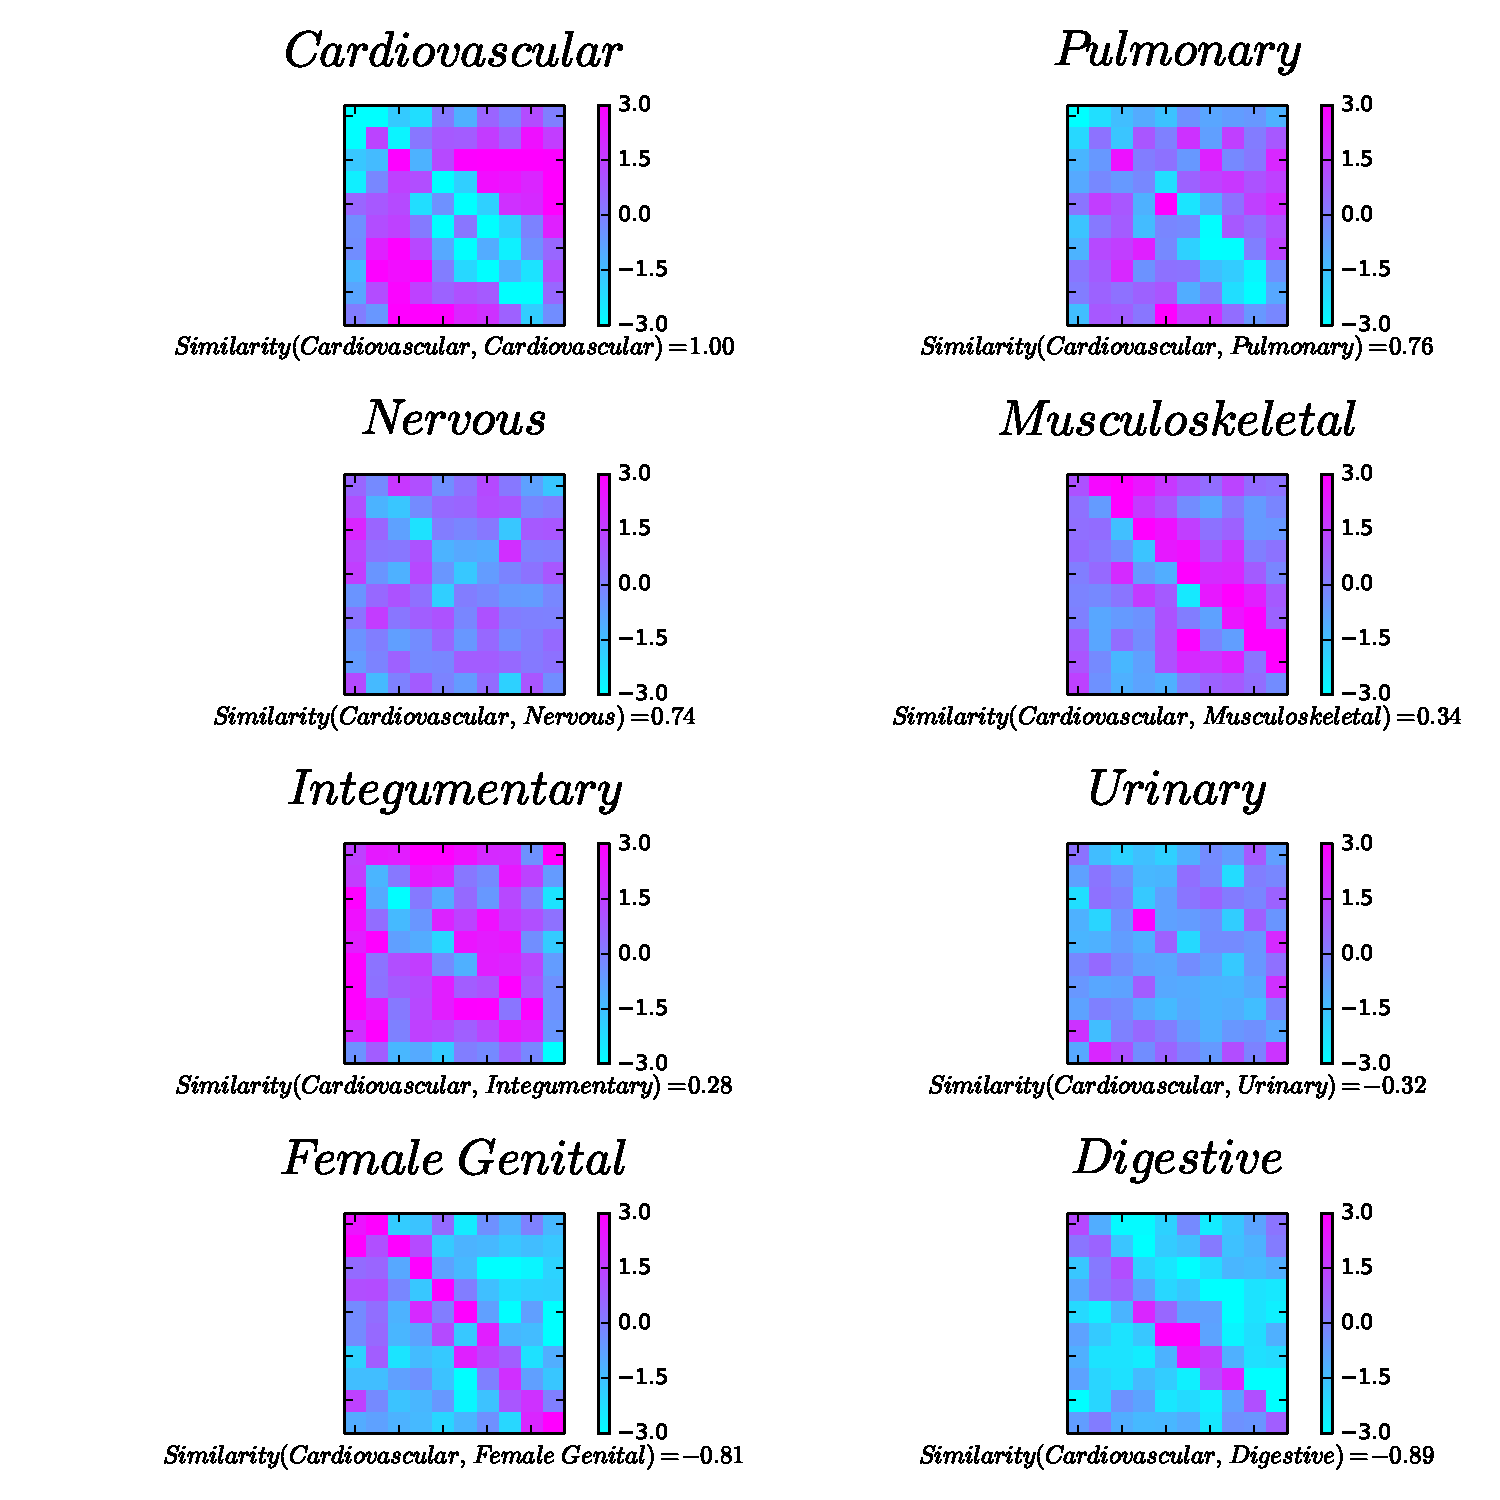
\includegraphics[scale=0.4]{./Figures/surgerytype_beta10.pdf}\\
  \caption{Icons for clusters of patients based on type of surgical procedure, $\beta=10$. Icons are sorted in descending similarity from the cluster of patients who underwent cardiovascular surgery.}\label{fig:surgerytype_beta10}
\end{figure}



\end{document} 